\documentclass{beamer}

\usepackage[francais]{babel}
\usepackage{rtxslides}
\usepackage{tikz}
\usetikzlibrary{shapes,fit}

\title{\rtx, \emph{THE} device driver generator}
\date[Soutenance Finale Ept4]{Soutenance Finale Ept4 \\ \vspace{10pt} 
\includegraphics[height=12mm]{logo_eip}}
\author[\rtx\ 2012 -- 16 juillet 2011]{\rtx\ 2012 -- 16 juillet 2011 \vspace{-20pt}}

\hypersetup{pdfauthor={Rathaxes 2012},pdfsubject={Rathaxes, THE device driver generator}}

\definecolor{lightred}{RGB}{147,36,33}
\tikzset{componentarrow/.style={<-, >=latex, color=rathaxesred, ultra thick}}

\newcommand{\cemph}[1]{{\itshape{\textcolor{rathaxesred}{#1}}}}

\newcommand{\bgcolor}{black}
\newcommand{\fgcolor}{white}

\tikzset{redbox/.style={draw,rectangle,rounded corners=5pt,ultra thick,color=rathaxesred,text=\fgcolor}}
\tikzset{warrow/.style={->, >=stealth, color=\fgcolor, ultra thick}}

\setbeamertemplate{navigation symbols}{}

\begin{document}

\begin{frame}
\titlepage
\end{frame}

\begin{frame}{Pilote de périphériques}
\begin{center}
\only<1>{
\textit{\rmfamily{\Huge{Avez vous déjà eu\ldots}}}
}

\only<2>{
\vspace{3mm}
\Large{un} \emph{\Huge{BSOD ?}}

\vspace{3mm}

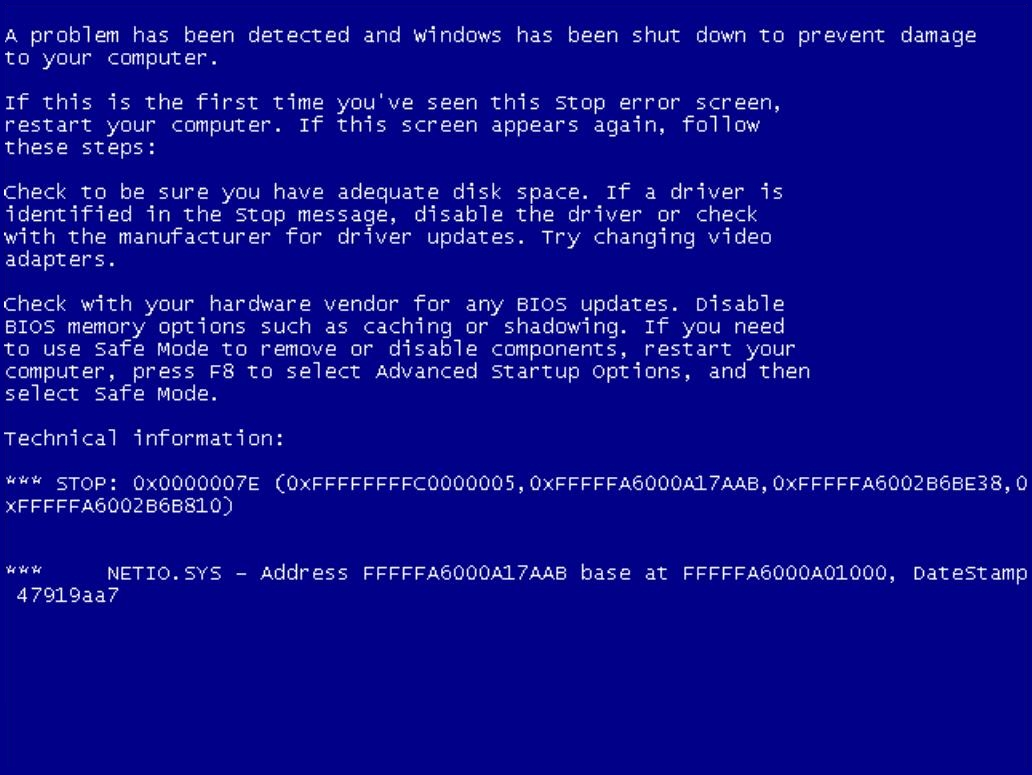
\includegraphics[width=80mm]{medias/bsod}
}

\only<3>{
\vspace{3mm}
\Large{ou un} \emph{\Huge{Kernel Panic ?}}

\vspace{3mm}

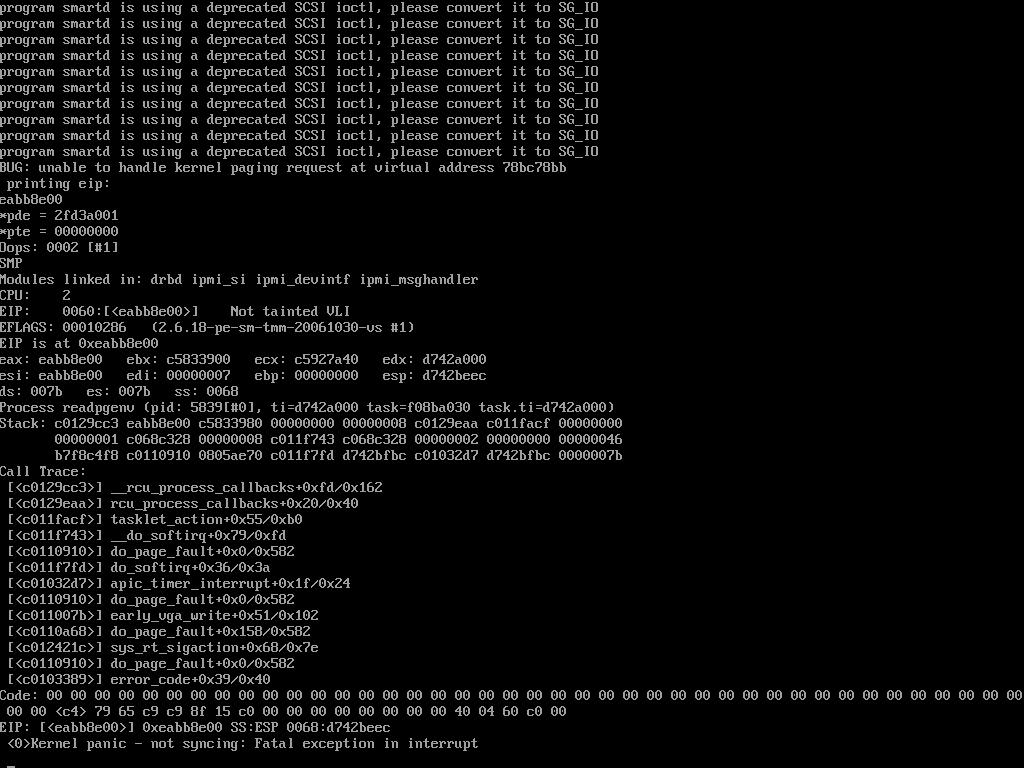
\includegraphics[width=80mm]{medias/panic}
}
\end{center}
\end{frame}

\begin{frame}{Quelques chiffres}
\Large{
\begin{itemize}
\setlength{\itemsep}{1em}
\item {\LARGE \emph{80 \%}} des rapports \cemph{d'erreurs} Windows \cemph{concernent les pilotes} de périphériques, selon Penny Orwick et Guy Smith ;
\item {\LARGE \emph{70 \%}} des \cemph{changements concernent les pilotes} dans chaque nouvelle version du noyau Linux.
\end{itemize}
}
\end{frame}

\begin{frame}{Les raisons}
\LARGE{
\begin{itemize}
\item Compétences requises ;
\item Rôle du code dans la machine.
\end{itemize}
}
\end{frame}

\begin{frame}{\rtx}
\LARGE{Le compilateur \rtx\ :}
\Large{
\vspace{1em}
\begin{itemize}
\item est la solution ;
\item démarré par une équipe diplômée en 2009.
\end{itemize}
}
\end{frame}

\begin{frame}[fragile]{Fonctionnement}
\begin{tikzpicture}[overlay]
\node (RTX) at (1,0) {
\includegraphics[height=1.5cm]{icons/rtx}};
\end{tikzpicture}
\end{frame}

\begin{frame}[fragile]{Fonctionnement}
\begin{tikzpicture}[overlay]
\node (RTX) at (1,0) {
\includegraphics[height=1.5cm]{icons/rtx}};

\node[redbox] (COMPILER) at (5.5,0) {\LARGE{Rathaxes}};

\draw[warrow] (RTX)--(COMPILER);
\end{tikzpicture}
\end{frame}

\begin{frame}[fragile]{Fonctionnement}
\begin{tikzpicture}[overlay]
\node (RTX) at (1,0) {
\includegraphics[height=1.5cm]{icons/rtx}};

\node[redbox] (COMPILER) at (5.5,0) {\LARGE{Rathaxes}};

\draw[warrow] (RTX)--(COMPILER);

\node (WDRV) at (10, 2.5) {
\includegraphics[height=2cm]{medias/driverbox}};

\node (LDRV) at (10, 0) {
\includegraphics[height=2cm]{medias/driverbox}};

\node (OTHER) at (10, -2.5) {
\includegraphics[height=2cm]{medias/driverbox}};

\draw (LDRV.north east) node[below left] {
\includegraphics[height=1.5cm]{medias/tux}};

\draw (WDRV.north east) node[below left] {
\includegraphics[height=1.3cm]{medias/windows_no_text}};

\draw (OTHER.north east) node[below left] {\Large{\ldots}};

\draw[warrow] (COMPILER.east)--(WDRV.south west);
\draw[warrow] (COMPILER.east)--(LDRV);
\draw[warrow] (COMPILER.east)--(OTHER.north west);
\end{tikzpicture}
\end{frame}

\begin{frame}{Fonctionnalités}
\begin{center}
\begin{tikzpicture}
\draw[fill=rathaxesred,color=rathaxesred,opacity=0.5,line width=0pt] (0, 0) circle (2.5);

\draw[fill=rathaxesred,color=rathaxesred,opacity=0.9,line width=0pt] (0, -1.5) circle (1);

\draw[warrow] (3, 1) -- (1, 1);
\draw[warrow] (3, -1.5) -- (1, -1.5);

\draw (3, 1) node[right] {\LARGE{Rathaxes 2012}};
\draw (3, -1.5) node[right] {\Large{Rathaxes 2009}};
\end{tikzpicture}
\end{center}
\end{frame}

\begin{frame}
\begin{center}
\emph{\Huge{Démonstration}}
\end{center}
\end{frame}

\begin{frame}[fragile]{Promotion}
\begin{center}
\begin{tikzpicture}
\node (RMLL) at (0, 0) {
\includegraphics[height=6cm]{rmll_2011}};

\draw (RMLL.east) node[right] {\begin{minipage}{45mm}\begin{itemize}
\item \Large{RMLL 2011} ;
\item \Large{Youtube} ;
\item \Large{Google Code} ;
\item \Large{Canal IRC}.
\end{itemize}\end{minipage}};
\end{tikzpicture}
\end{center}
\end{frame}

\begin{frame}{Objectifs pour la 5ème année}
\Large{
\begin{itemize}
\setlength{\itemsep}{1em}
\item Écriture du code pour chaque plateforme ;
\item Intégration continue.
\end{itemize}
}
\end{frame}

\begin{frame}[fragile]{Groupe}
\begin{center}
\begin{tikzpicture}[overlay]
\node[redbox] (ZOBI) at (0, 2) {\begin{minipage}{46mm}\begin{center}Thomas Luquet \\ \small{\emph{Responsable du groupe}}\end{center}\end{minipage}};

\node[redbox] (ZO) at (-3, 0) {\begin{minipage}{46mm}\begin{center}Zoltan Konarzweski \\ \small{\emph{Langage \& Compilateur}}\end{center}\end{minipage}};
\node[redbox] (JOA) at (3, 0) {\begin{minipage}{46mm}\begin{center}David Pineau \\ \small{\emph{Langage \& Compilateur}}\end{center}\end{minipage}};

\node[redbox] (KAL) at (-3, -2) {\begin{minipage}{46mm}\begin{center}Louis Opter \\ \small{\emph{Pilotes Unix \& Mainteneur}}\end{center}\end{minipage}};
\node[redbox] (DAEDRIC) at (3, -2) {\begin{minipage}{46mm}\begin{center}Thomas Sanchez \\ \small{\emph{Pilotes Unix \& Windows}}\end{center}\end{minipage}};
\end{tikzpicture}
\end{center}
\end{frame}

\begin{frame}{Merci}
\begin{center}
\Huge{\emph{Questions ?}}
\end{center}

\vspace{2em}
\begin{itemize}
\item \Large{\texttt{http://www.rathaxes.org/}}
\end{itemize}
\end{frame}

\setbeamertemplate{footline}{}

\begin{frame}[fragile]
\begin{center}
\begin{tikzpicture}[overlay]
\node (RTX) at (-1,0.5) {
\includegraphics[height=60mm]{logo_latex}};

\draw (0, -3.3) node {\Huge{\cemph{Rathaxes}}};

\draw (5.3, -4.6) node {
\includegraphics[height=7mm]{logo_eip}};

\draw (3.5, -4.6) node {
\includegraphics[height=7mm]{logo_epitech}};
\end{tikzpicture}
\end{center}
\end{frame}

\end{document}
